\documentclass{article}

\def\MyClass{Álgebra Lineal}
\def\MyTitle{Taller 3}
\def\MyAuthor{Martín Steven Hernández Ortiz}
\def\MyEmail{mahernandezor@unal.edu.co}
\def\MyDate{\today}

\def\TemplatePath{../template/}

%%% Template Packages %%%

\usepackage{graphicx} % Images
\usepackage{tcolorbox} % Color Box
\usepackage[%
vmargin=2.25cm,%
hmargin=2.25cm%
]{geometry} % Page Geometry
\usepackage{fancyhdr} % Header / Footer Styles
\usepackage{extramarks} % Header / Footer Marks

\usepackage{ragged2e} % Text Align
\usepackage{amsmath} % Math Align

\usepackage{booktabs} % Tables+ Package
\usepackage{enumitem} % Enumarete+ Package

\usepackage{mathtools} % Math General
\usepackage{amsthm} % Math Envs
\usepackage{unicode-math} % Math Symbols

\usepackage{polyglossia} % Language
    \setdefaultlanguage{spanish}

\renewcommand{\thefootnote}{\Roman{footnote}} % Changing footnotes arabic to roman numbers

%%% Template Styles %%%

% Header / Footer Styles
\pagestyle{fancy}
\RenewDocumentCommand{\headrule}{}{%
    \rule[0.1cm]{\textwidth}{0.1mm}%
}
\RenewDocumentCommand{\footrule}{}{%
    \rule[0.1cm]{\textwidth}{0.1mm}%
}

\fancyhf[HC]{{\slshape \MyTitle{}}}
\fancyhead[HL]{\firstleftxmark}
\fancyhead[HR]{\lastleftxmark}

% Redefine \maketitle
\RenewDocumentCommand{\maketitle}{s}{%
    \begin{@twocolumntrue}%
        \begin{minipage}{0.3\textwidth}%
            \begin{Center}
                
\includegraphics[width=0.6\textwidth]{../template/src/unal_logo.pdf}%
            \end{Center}
        \end{minipage}%
        \begin{minipage}{0.7\textwidth}{{%
        \begin{Center}%
            {\large \itshape \MyClass{}} \\[1ex]
            {\huge  \slshape \MyTitle{}} \\[4ex]
            {\Large  \MyAuthor{}} \\[0ex]
            {\small  \MyEmail{}} \\[4ex] 
            \MyDate{}
        \end{Center}%
        }}%
        \end{minipage}%
    \end{@twocolumntrue}%
    \vspace{0.5cm}%
    \begin{Center}%
        \rule[0cm]{\textwidth}{0.1mm}%
    \end{Center}%
    \vspace{0.5cm}%
}

% Enumerate Lists types
\newcommand{\listSubscript}[2]{\(#1_{#2}\)}
\newcommand{\listAlph}{(\alph*)}

%%% Template Math stuff %%%

% Theorems
\newtheorem{TMPMathTheorem}{Teorema}
\NewDocumentEnvironment{theorem}{+b} {%
    \begin{TMPMathTheorem}%
        #1 %
    \end{TMPMathTheorem}%
} {}

% Collorary
\newtheorem{TMPMathCorollary}[TMPMathTheorem]{Corolario}
\NewDocumentEnvironment{corollary}{+b} {%
    \begin{TMPMathCorollary}%
        #1 %
    \end{TMPMathCorollary}%
} {}

% Definitions
\newtheorem{TMPMathDefinition}[TMPMathTheorem]{Definición}
\NewDocumentEnvironment{definition}{+b} {%
    \begin{tcolorbox}[left=0mm,right=0mm]%
        \begin{TMPMathDefinition}%
            #1 %
            \begin{FlushRight}%
                \(\bigtriangleup{}\)%
            \end{FlushRight}%
        \end{TMPMathDefinition}%
    \end{tcolorbox}%
} {}



\def\fancyL{\symscr{L}}
\def\fancyP{\symscr{P}}
\def\realR{\symbb{R}}
\def\realN{\symbb{N}}

\begin{document}
\maketitle
\begin{enumerate}
    \item Un punto \(P\) pertenece a la recta que pasa por los puntos \(\left(\begin{smallmatrix}4 \\ 2 \\ 2\end{smallmatrix}\right)\) y \(\left(\begin{smallmatrix}-2 \\ 0 \\ 6\end{smallmatrix}\right)\), si la coordenada \(y\) de \(P\) es 1, hallar sus otras coordenadas. \\
        Primero definamos una ecuación vectorial de la recta que pasa por \(\left(\begin{smallmatrix}4 \\ 2 \\ 2\end{smallmatrix}\right)\) y \(\left(\begin{smallmatrix}-2 \\ 0 \\ 6\end{smallmatrix}\right)\)        
        \[
            \begin{aligned}
                A &= \begin{pmatrix}4 \\ 2 \\ 2\end{pmatrix} \\
                B &= \begin{pmatrix}-2 \\ 0 \\ 6\end{pmatrix} 
            \end{aligned}
            \hspace{0.5cm}
            \text{;}
            \hspace{0.5cm}
            \overline{AB} = \begin{pmatrix}-6 \\ -2 \\ 4\end{pmatrix}
            \hspace{0.5cm}
            \text{;}
            \hspace{0.5cm}
            \fancyL :
            \begin{pmatrix}x \\ y \\ z\end{pmatrix}
                =
            \begin{pmatrix}4 \\ 2 \\ 2\end{pmatrix}
                +
            t \cdot \begin{pmatrix}-6 \\ -2 \\ 4\end{pmatrix}
        \]
        Ahora, si \(P\) es un punto que pasa por \(\fancyL\) entonces va a existir un \(t\) tal que para las ecuaciones parámetricas de \(\fancyL\)
        se pueda reemplazar las coordenadas de \(P\) en las variables de cada ecuación. Sin embargo, por ahora, solo nos vamos a concentrar en la 2\tsup{da} ecuación parámetrica.
        \[
            P = \begin{pmatrix}a \\ 1 \\ c\end{pmatrix}
            \hspace{1cm}
            \left\{
            \begin{aligned}
                a &= 4 + -6t \\
                1 &= 2 + -2t \\
                c &= 2 + 4t
            \end{aligned}
            \right.
            \hspace{0.5cm}
            \text{;}
            \hspace{0.5cm}
            -1 = -2t
            \hspace{0.5cm}
            \text{;}
            \hspace{0.5cm}
            \frac{1}{2} = t
            \hspace{0.5cm}
        \]
        Ahora, veamos que valores de \(a\) y \(c\) vamos a tener con este valor de \(t\)
        \[
            \left\{
            \begin{aligned}
                a &= 4 + -6\left(\frac{1}{2}\right) \\
                c &= 2 + 4\left(\frac{1}{2}\right)
            \end{aligned}
            \right.
            \hspace{0.5cm}
            \text{;}
            \hspace{0.5cm}
            \left\{
                \begin{aligned}
                    a &= \frac{8}{2} + -\frac{6}{2} \\
                    c &= \frac{4}{2} + \frac{4}{2}
                \end{aligned}
            \right.
            \hspace{0.5cm}
            \text{;}
            \hspace{0.5cm}
            \left\{
                \begin{aligned}
                    a &= \frac{2}{2} = 1 \\
                    c &= \frac{8}{2} = 4
                \end{aligned}
            \right.
        \]
        Entonces, vamos a tener que \(P\) es el punto 
        \(
            \begin{pmatrix}
                1 \\ 1 \\ 4
            \end{pmatrix}
        \)
    \item Hallar la ecuación de la recta que pasa por \(\left(\begin{smallmatrix}2 \\ 1 \\ 5\end{smallmatrix}\right)\) y corta en forma perpendicular a la recta dada por las ecuaciones simétricas:
        \[
            \frac{x - 1}{3} = \frac{y + 2}{4} = \frac{z - 3}{2}
        \]
        Primero, encontremos el vector director de la recta dada por ecuaciones simétricas
        \[
            \fancyL_1 : 
            \begin{pmatrix}
                x \\ y \\ z
            \end{pmatrix} =
            \begin{pmatrix}
                1 \\ -2 \\ 3
            \end{pmatrix}
            + 
            t \cdot
            \begin{pmatrix}
                3 \\ 4 \\ 2
            \end{pmatrix}
            \hspace{1cm}
            \text{;}
            \hspace{1cm}
            d_1 = 
            \begin{pmatrix}
                3 \\ 4 \\ 2
            \end{pmatrix}
        \]
        Ahora, busquemos la ecuación normal del Hiperplano teniendo a \(d_1\) como vector normal para así apartir de \(\left(\begin{smallmatrix}2 \\ 1 \\ 5\end{smallmatrix}\right)\)
        poder encontrar un vector ortogonal tal que corte en un punto a \(\fancyL_1\), y que pase por \(\left(\begin{smallmatrix}2 \\ 1 \\ 5\end{smallmatrix}\right)\). 
        Donde, \(A\) va a ser el punto donde corte el vector ortogonal a \(\fancyL_1\), se va a tener
        \[
            \begin{aligned}
                \left(
                    A 
                    - 
                    \begin{pmatrix}
                        2 \\ 1 \\ 5 
                    \end{pmatrix}
                \right)
                \cdot 
                \begin{pmatrix}
                    3 \\ 4 \\ 2
                \end{pmatrix}
                &= 0 \\
                    A 
                \cdot 
                \begin{pmatrix}
                    3 \\ 4 \\ 2
                \end{pmatrix}
                -
                \begin{pmatrix}
                    2 \\ 1 \\ 5 
                \end{pmatrix}
                \cdot 
                \begin{pmatrix}
                    3 \\ 4 \\ 2
                \end{pmatrix}
                &= 0 \\
                A 
                \cdot 
                \begin{pmatrix}
                    3 \\ 4 \\ 2
                \end{pmatrix}
                &=
                \begin{pmatrix}
                    2 \\ 1 \\ 5 
                \end{pmatrix}
                \cdot 
                \begin{pmatrix}
                    3 \\ 4 \\ 2
                \end{pmatrix}
                = 20
            \end{aligned}
        \]
        Entonces vamos a necesitar que el producto punto de \(A\) y \(\left(\begin{smallmatrix}3 \\ 4 \\ 2\end{smallmatrix}\right)\) sea igual a 20. 
        Y más importante, también que \(A\) este en \(\fancyL_1\), ya que es lo importante en este problema. 
        Entonces, debe existir un escalar \(\lambda\) tal que \(A\) va a ser un punto en \(\fancyL_1\) y al mismo tiempo, 
        el producto punto del mismo \(A\) con \(\left(\begin{smallmatrix}2 \\ 1 \\ 5\end{smallmatrix}\right)\) va a ser 20.
        \[
            A = 
            \begin{pmatrix}
                a_1 \\ a_2 \\ a_3
            \end{pmatrix}
            \hspace{0.5cm}
            \text{;}
            \hspace{0.5cm}
            \begin{cases}
                a_1 = 1 + 3\lambda \\ 
                a_2 = -2 + 4\lambda \\ 
                a_3 = 3 + 2\lambda
            \end{cases}
            \hspace{0.5cm}
            \wedge
            \hspace{0.5cm}
            3a_1 + 4a_2 + 2a_3 = 20
        \]
        \[
            \begin{aligned}
                3a_1 + 4a_2 + 2a_3 &= 20 \\
                3(1 + 3\lambda) + 4(-2 + 4\lambda) + 2(3 + 2\lambda) &= 20 \\
                3 + 9\lambda -8 + 16\lambda + 6 + 4\lambda &= 20 \\
                1 + 29\lambda &= 20 \\
                29\lambda &= 20 - 1\\
                \lambda &= \frac{19}{29}\\
            \end{aligned}
            \hspace{1cm}
            \begin{aligned}
                A &=
                \begin{pmatrix}
                    1 \\ -2 \\ 3
                \end{pmatrix}
                +
                \left(
                    \frac{19}{29}
                \right)
                \cdot
                \begin{pmatrix}
                    3 \\ 4 \\ 2
                \end{pmatrix} \\
                &=
                \begin{pmatrix}
                    1 \\ -2 \\ 3
                \end{pmatrix}
                +
                \begin{pmatrix}
                    \frac{57}{29} \\ \frac{76}{29} \\ \frac{38}{29}
                \end{pmatrix} \\
                &=
                \begin{pmatrix}
                    \frac{86}{29} \\ \frac{18}{29} \\ \frac{125}{29}
                \end{pmatrix} \\
            \end{aligned}
        \]
        Ahora que tenemos todos los componentes necesarios para crear a \(\fancyL_2\), una recta tal que pase por \(\left(\begin{smallmatrix}2 \\ 1 \\ 5\end{smallmatrix}\right)\)
        y sea ortogonal con la recta \(\fancyL_1\) la podremos graficar, vease Figura-\ref{pt-two-graph}.
        \[
            \fancyL_2 :
            \begin{pmatrix}
                x \\ y \\ z 
            \end{pmatrix}
            =
            \begin{pmatrix}
                2 \\ 1 \\ 5
            \end{pmatrix}
            +
            t
            \cdot
            \begin{pmatrix}
                \frac{86}{29} \\ \frac{18}{29} \\ \frac{125}{29}
            \end{pmatrix}
        \]
        \begin{figure}
            \centering
            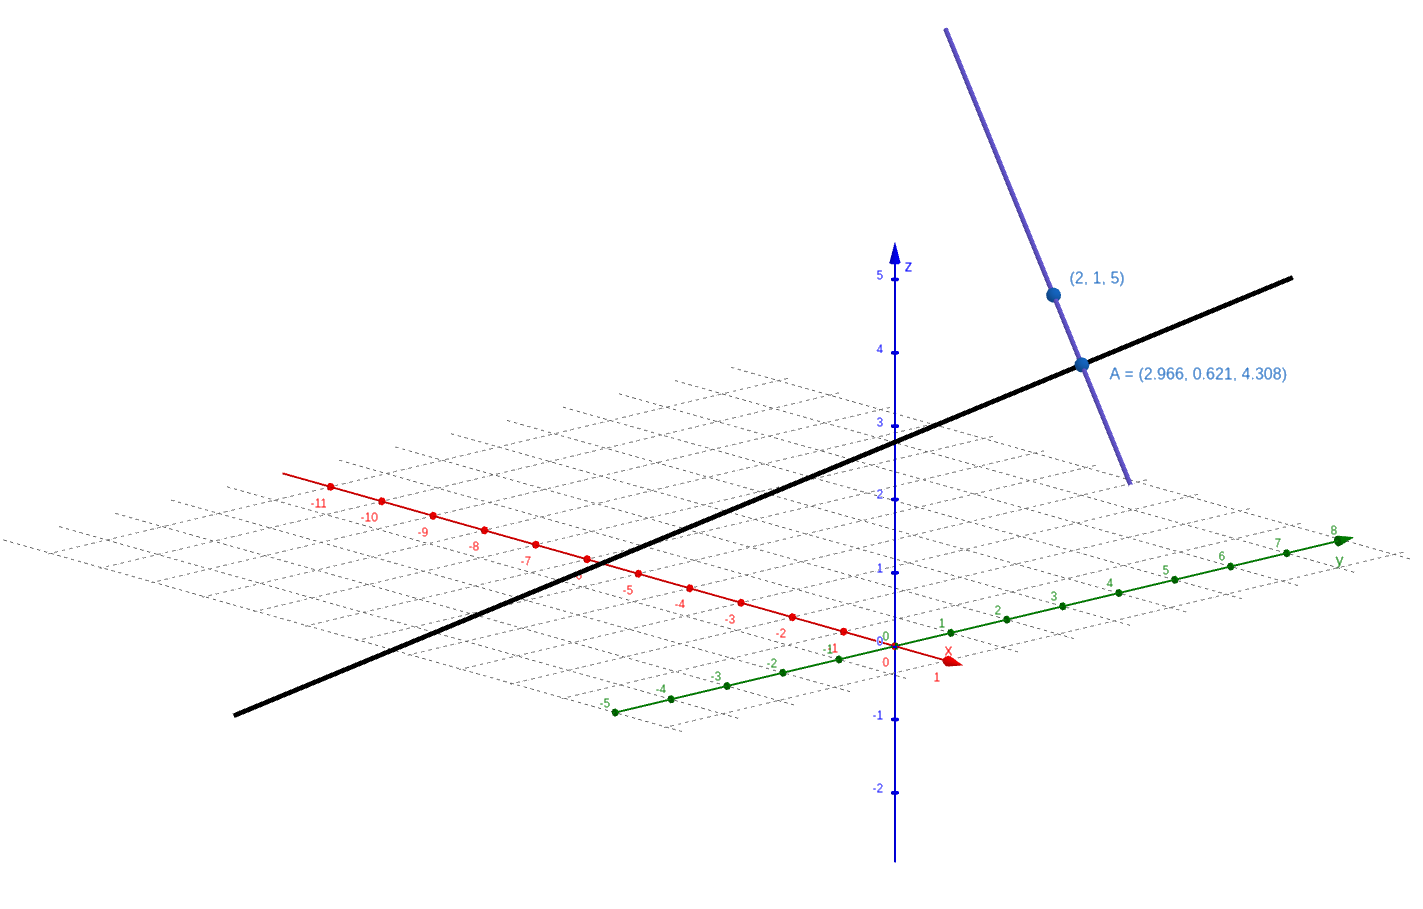
\includegraphics[width=15cm]{src/2_lines.png}
            \caption{Grafica de \(\fancyL_1\) y \(\fancyL_2\) del punto 2 en \(\realR^3\)}%
            \label{pt-two-graph}
        \end{figure}
    \setcounter{enumi}{5}
    \item Muestre que las rectas 
        \[
            \fancyL{}_1:
            \left\{
            \begin{aligned}
                x &= 2 − t,\\
                y &= 1 + t,\\
                z &= −2t
            \end{aligned}
            \right.
            \hspace{1cm}
            \text{y}
            \hspace{1cm}
            \fancyL{}_2:
            \left\{
            \begin{aligned}
                x &= 1 + s,\\
                y &= −2s,\\
                z &= 3 + 2s
            \end{aligned}
            \right.
        \]
        no tienen puntos en común. \\
        Primero, miremos si ambas rectas son paralelas, es decir si el vector director de una recta es una múltiplo por escalar del otro vector director.
        \[
            \lambda
            \begin{pmatrix}
                -1 \\ 1 \\ -2
            \end{pmatrix}
            =
            \begin{pmatrix}
                1 \\ -2 \\ 2
            \end{pmatrix}
            \hspace{1cm}
            \begin{cases}
                -\lambda = 1 \\
                \lambda = -2 \\
                -2\lambda = 2
            \end{cases}
            \hspace{0.5cm}
            \begin{cases}
                \lambda = -1 \\
                \lambda = -2 \\
                \lambda = -1
            \end{cases}
        \]
        Dado que, para que \(\fancyL_1\) y \(\fancyL_2\) sean paralelas, \(\lambda\) tiene que ser consistente, entonces vamos a tener que \(\fancyL_1 \nparallel \fancyL_2\).
        Ahora, veamos si ambias rectas son perpendiculares, para así tener más información de estás.
        \[
            d_1 \cdot d_2 = 
            \begin{pmatrix}
                -1 \\ 1 \\ -2 
            \end{pmatrix}
            \cdot
            \begin{pmatrix}
                1 \\ -2 \\ 2
            \end{pmatrix}
            =
            (-1 \cdot 1) + (1 \cdot -2) + (-2 \cdot 2)
            = 
            -1 -2 -4
            = 
            -6
        \]
        De manera similar, tenemos que el producto punto de los vectores directores de \(\fancyL_1\) y \(\fancyL_2\) no es 0. Entonces \(\fancyL_1 \not\perp \fancyL_2\).
        Entre tanto, para verificar que \(\fancyL_1\) y \(\fancyL_2\) no interseccionen en ningún punto, se va a igualar ambas ecuaciones vectoriales,
        y apartir de este punto, mirar cada ecuación parámetrica. Esto ya que, 
        para que dos rectas tengan una intersección en un punto es necesario que exista un \(t\) y \(s\) para cada recta tal que sean iguales a el punto.
        \[
            \begin{aligned}
                \begin{pmatrix}
                    x \\ y \\ z
                \end{pmatrix}
                =
                \begin{pmatrix}
                    2 \\ 1 \\ 0
                \end{pmatrix}
                +
                t
                \begin{pmatrix}
                    -1 \\ 1 \\ -2
                \end{pmatrix}
                &=
                \begin{pmatrix}
                    1 \\ 0 \\ 3
                \end{pmatrix}
                +
                s
                \begin{pmatrix}
                    1 \\ -2 \\ 2
                \end{pmatrix} \\
                \begin{cases}
                    x = 2 -t \\
                    y = 1 + t \\
                    z = -2t
                \end{cases}
                &=
                \begin{cases}
                    x = 1 + s \\
                    y = -s \\
                    z = 3 + 2s
                \end{cases} \\
            \end{aligned}
        \]
        \[
            \begin{cases}
                2 -t = x = 1 + s \\
                1 + t = y = -s \\
                -2t = z = 3 + 2s
            \end{cases}
            \hspace{1cm}
            \begin{cases}
                t = 1 - s \\
                t = -1 - s \\
                t = -\frac{3}{2} - s
            \end{cases}
            \hspace{0.5cm}
            \text{;}
            \hspace{0.5cm}
            \begin{cases}
                2 -t = x = 1 + s \\
                1 + t = y = -s \\
                -2t = z = 3 + 2s
            \end{cases}
            \hspace{1cm}
            \begin{cases}
                1 -t = s \\
                -1 - t = s \\
                -\frac{3}{2} - t = s
            \end{cases}
        \]
        Como resultado se puede ver que no existe un valor consistente de \(t\) y \(s\) tal que \(\fancyL_1\) y \(\fancyL_2\) tengan un punto en común.

%\item Acerca de los planos \(\fancyP{}_1: 2x − y + z = 3\) y \(\fancyP{}_2: x + y − z = 7\), es correcto afirmar que estos son:
    %\begin{enumerate}[label=\listAlph]
        %\item Paralelos
        %\item Ortogonales
        %\item El mismo
        %\item N.A
    %\end{enumerate}

%\setcounter{enumi}{9}
%\item Encuentre dos puntos y dos vectores directores de la recta de \(\realR^4\), \(\fancyL = \frac{x + 5}{-3} = 1 + z = \frac{w}{3}, y = 0\).
%\setcounter{enumi}{13}
%\item Determine si la recta \(\fancyL = \frac{x + 5}{-3} = 1 + z = \frac{w}{2}, y = 0\) intercepta a cada uno de los siguientes planos
    %\[
        %\fancyP_1 = 
        %\begin{cases}
            %x = 1 - 2t \\
            %y = 2t - 4s \\
            %z = -3t + 7s \\
            %w = 4t - 6s
        %\end{cases}
        %\hspace{1cm}
        %\text{y}
        %\hspace{1cm}
        %\fancyP_2 = 
        %\begin{cases}
            %x = -t -s \\
            %y = 5t - 6s \\
            %z = -4t + 4s \\
            %w = -4
        %\end{cases}
    %\]
    %En caso afirmativo, encuentre la intersección.
%\item Dadas las ecuaciones de las rectas \(\fancyL_1, \fancyL_2\) y de los planos \(\fancyP_1, \fancyP_2\)
    %\[
        %\begin{aligned}
            %\fancyL_1 &= 
            %\begin{cases}
                %x = 3 + t \\
                %y = 2 - 2t \\
                %z = 2t \\
                %w = 0
            %\end{cases}
            %\hspace{1cm}
            %&\text{y}
            %\hspace{1cm}
            %\fancyL_2 &:
            %\frac{x - 2}{-1} =
            %\frac{y - 3}{2} =
            %\frac{z + 2}{-2}, w = 0 \\
            %\fancyP_1 &=
            %\begin{cases}
                %x = 2 + 4t \\
                %y = -2 + t + 2s \\
                %z = 1 -t + 2s \\
                %w = 3 + 3t
            %\end{cases}
            %\hspace{1cm}
            %&\text{y}
            %\hspace{1cm}
            %\fancyP_2 &=
            %\begin{cases}
                %w = 6 - t - 3s \\
                %y = 2 + s \\
                %z = -6 + 2t + 2s \\
                %w = -3 + t + 2s
            %\end{cases}
        %\end{aligned}
    %\]
    %Determine cuáles de las siguientes afirmaciones son \textbf{VERDADERAS} y cuáles \textbf{FALSAS}
%\item Sean \(\fancyL_1, \fancyL_2, \fancyL_3\) y \(\fancyP_1, \fancyP_2, \fancyP_3\) las siguientes rectas y planos de \(\realR^3\) y \(P\) un punto en \(\realR^3\)
    %\[
        %\begin{aligned}
            %\fancyL_1 &=
            %\begin{cases}
                %x = -t \\
                %y = 1 + 2t \\
                %z = -2 + 3t
            %\end{cases} \\
            %\fancyL_2 &=
            %\frac{x + 5}{6} =
            %\frac{z - 1}{2},
            %y = -1 \\
            %\fancyL_3 &: 
            %\begin{pmatrix}x \\ y \\ z\end{pmatrix}
            %=
            %\begin{pmatrix}0 \\ -1 \\ 2\end{pmatrix}
            %+
            %t\begin{pmatrix}3 \\ 1 \\ -1\end{pmatrix}
        %\end{aligned}
        %\hspace{1cm}
        %\text{y}
        %\hspace{1cm}
        %\begin{aligned}
            %\fancyP_1 &=
            %\begin{cases}
                %x = -3 -2t \\
                %y = 5t - 6s \\ 
                %z = 1 - 4t + 4s
            %\end{cases} \\
            %\fancyP_2 &:
            %x - 4y + 3z - 7 = 0 \\ 
            %\fancyP_3 &:
            %\begin{pmatrix}x_1 \\ x_2 \\ x_3\end{pmatrix}
            %=
            %\begin{pmatrix}-1 \\ 0 \\ 2\end{pmatrix}
            %+ t\begin{pmatrix}3 \\ -3 \\ -5\end{pmatrix}
            %+ s\begin{pmatrix}6 \\ 0 \\ -2\end{pmatrix}
        %\end{aligned}
    %\]
    %\[
        %P = \begin{pmatrix}
            %1 \\ -2 \\ 3
        %\end{pmatrix}
    %\]
    %\begin{enumerate}[label=\listAlph]
		%\item Encuentre un punto de cada recta y cada plano.
            %\[
                %\begin{aligned}
                    %\fancyL_1:&
                    %t = 1;
                    %\begin{cases}
                        %x = -1 \\
                        %y = 1 + 2 = 3 \\
                        %z = -2 + 3 = 1
                    %\end{cases};
                    %\hspace{0.5cm}
                    %&
                    %\begin{pmatrix}
                        %-1 \\ 3 \\ 1
                    %\end{pmatrix}
                    %\in \fancyL_1
                    %\\
                    %\fancyL_2:&
                    %t = 1;
                    %\frac{x + 5}{6} =
                    %\frac{z - 1}{2} = 1,
                    %y = -1;
                    %\hspace{0.5cm}
                    %\begin{aligned}
                        %\frac{x + 5}{6} &= 1 \\
                        %\frac{z - 1}{2} &= 1 \\
                    %\end{aligned};
                    %\hspace{0.5cm}
                    %\begin{aligned}
                        %x &= 6 - 5 = 1 \\
                        %z &= 2 + 1 = 3 \\
                    %\end{aligned};
                    %\hspace{0.5cm}
                    %&
                    %\begin{pmatrix}
                        %1 \\ -1 \\ 3
                    %\end{pmatrix}
                    %\in \fancyL_2
                    %\\
                    %\fancyL_3:&
                    %t = 1;
                    %\begin{pmatrix}0 \\ -1 \\ 2\end{pmatrix}
                    %+
                    %\begin{pmatrix}3 \\ 1 \\ -1\end{pmatrix}
                    %=
                    %\begin{pmatrix}3 \\ 0 \\ 1\end{pmatrix};
                    %\hspace{0.5cm}
                    %&\begin{pmatrix}3 \\ 0 \\ 1\end{pmatrix}
                    %\in \fancyL_3
                    %\\
                    %\fancyP_1:&
                    %\begin{aligned}
                        %t &= 1 \\
                        %s &= 1
                    %\end{aligned};
                    %\begin{cases}
                        %x = -3 -2 = -5 \\
                        %y = 5 - 6 = -1 \\ 
                        %z = 1 - 4 + 4 = 1
                    %\end{cases};
                    %\hspace{0.5cm}
                    %&
                    %\begin{pmatrix}
                        %-5 \\ -1 \\ 1
                    %\end{pmatrix}
                    %\in \fancyP_1
                    %\\
                    %\fancyP_2:&
                    %\begin{aligned}
                        %x &= 0 \\
                        %y &= -1 \\
                        %z &= 1 \\
                    %\end{aligned};
                    %\begin{aligned}
                        %x − 4y + 3z − 7 &= 0 \\
                        %x − 4y + 3z &= 7
                    %\end{aligned}
                    %\hspace{0.5cm}
                    %\begin{aligned}
                        %−4(-1) + 3(1) &= 7 \\
                        %7 &= 7
                    %\end{aligned}
                    %&
                    %\begin{pmatrix}
                        %0 \\ -1 \\ 1
                    %\end{pmatrix}
                    %\in
                    %\fancyP_2
                    %\\
                    %\fancyP_3:&
                    %\begin{aligned}
                        %t &= 1 \\
                        %s &= 1
                    %\end{aligned};
                    %\begin{pmatrix}x_1 \\ x_2 \\ x_3\end{pmatrix}
                    %=
                    %\begin{pmatrix}-1 \\ 0 \\ 2\end{pmatrix}
                    %+ \begin{pmatrix}3 \\ -3 \\ -5\end{pmatrix}
                    %+ \begin{pmatrix}6 \\ 0 \\ -2\end{pmatrix}
                    %=
                    %\begin{pmatrix}8 \\ -3 \\ -5\end{pmatrix}
                    %&
                    %\begin{pmatrix}
                        %8 \\ -3 \\ -5
                    %\end{pmatrix}
                    %\in \fancyP_3
                %\end{aligned}
            %\]
		%\item Encuentre un vector director de cada recta. \\
            %\[
                %\fancyL_1:
                %d_1 =
                %\begin{pmatrix}
                    %-1 \\ 2 \\ 3
                %\end{pmatrix}
                %\hspace{1.5cm}
                %\fancyL_2:
                %d_2 =
                %\begin{pmatrix}
                    %6 \\ 0 \\ 2
                %\end{pmatrix}
                %\hspace{1.5cm}
                %\fancyL_3:
                %d_3 =
                %\begin{pmatrix}
                    %3 \\ 1 \\ -1
                %\end{pmatrix}
            %\]
		%\item Encuentre los otros dos tipos de ecuaciones de las rectas.
            %\[
                %\begin{aligned}
                    %&\fancyL_1
                    %\begin{aligned}
                        %&:\begin{pmatrix}
                            %x \\ y \\ z
                        %\end{pmatrix} 
                        %= 
                        %\begin{pmatrix}
                            %0 \\ 1 \\ -2
                        %\end{pmatrix}
                        %+
                        %t\begin{pmatrix}
                            %-1 \\ 2 \\ 3
                        %\end{pmatrix};
                        %\hspace{0.5cm}
                        %t \in \realR
                        %\\
                        %&=
                        %-x
                        %=
                        %\frac{y - 1}{2}
                        %=
                        %\frac{z + 2}{3}
                    %\end{aligned}
                    %\hspace{0.5cm}
                    %&\fancyL_2
                    %\begin{aligned}
                        %&:\begin{pmatrix}
                            %x \\ y \\ z
                        %\end{pmatrix} 
                        %= 
                        %\begin{pmatrix}
                            %-5 \\ -1 \\ 1
                        %\end{pmatrix}
                        %+
                        %t\begin{pmatrix}
                            %6 \\ 0 \\ 2
                        %\end{pmatrix};
                        %\hspace{0.5cm}
                        %t \in \realR
                        %\\
                        %&= \begin{cases}
                            %x = -5 + 6t\\
                            %y = -1\\ 
                            %z = 1 + 2t\\
                        %\end{cases};
                        %\hspace{0.5cm}
                        %t \in \realR
                    %\end{aligned}
                    %\\[0.5cm]
                    %&\fancyL_3
                    %\begin{aligned}
                        %&= \begin{cases}
                            %x = 3t\\
                            %y = -1 + t\\ 
                            %z = 2 - t\\
                        %\end{cases}
                        %\hspace{0.5cm}
                        %t \in \realR
                        %\\
                        %&=
                        %\frac{x}{3}
                        %=
                        %y + 1
                        %=
                        %-z + 2
                    %\end{aligned}
                %\end{aligned}
            %\]
		%\item Encuentre dos vectores directores de cada plano.
            %\[
                %\begin{aligned}
                    %\fancyP_1:&
                    %\hspace{0.5cm}
                    %t_1 = \begin{pmatrix}
                        %-2 \\ 5 \\ -4
                    %\end{pmatrix}
                    %\hspace{0.5cm}
                    %s_1 = \begin{pmatrix}   
                        %0 \\ -6 \\ 4
                    %\end{pmatrix}
                    %\\
                    %\fancyP_2:&
                    %\hspace{0.5cm}
                    %t_2 = \begin{pmatrix}
                    %\end{pmatrix}
                    %\hspace{0.5cm}
                    %s_2 = \begin{pmatrix}
                    %\end{pmatrix};
                    %\\
                    %\fancyP_3:&
                    %\hspace{0.5cm}
                    %t_3 = \begin{pmatrix}
                        %3 \\ -3 \\ -5
                    %\end{pmatrix}
                    %\hspace{0.5cm}
                    %s_3 = \begin{pmatrix}
                        %6 \\ 0 \\ -2
                    %\end{pmatrix}
                %\end{aligned}
            %\]
		%\item Encuentre un vector normal de cada plano.
            %\[
                %\begin{aligned}
                    %\fancyP_1:&
                    %\hspace{0.5cm}
                    %\begin{aligned}
                        %n_1 &= 
                        %\begin{pmatrix}
                            %-2 \\ 5 \\ -4
                        %\end{pmatrix}
                        %\times
                        %\begin{pmatrix}
                            %0 \\ -6 \\ 4
                        %\end{pmatrix}
                        %=
                        %\begin{pmatrix}
                            %(5 \cdot 4) - (-4 \cdot -6) \\
                            %- ((-2 \cdot 4) - (-4 \cdot 0)) \\
                            %(-2 \cdot -6) - (5 \cdot 0)
                        %\end{pmatrix}
                        %\\
                        %&=
                        %\begin{pmatrix}
                            %20 - 24 \\
                            %- (-8 - 0) \\
                            %12 - 0
                        %\end{pmatrix}
                        %=
                        %\begin{pmatrix}
                            %-4 \\ 8 \\ 12
                        %\end{pmatrix}
                    %\end{aligned}
                    %\hspace{0.5cm}
                    %\fancyP_2:&
                    %\hspace{0.5cm}
                    %n_2 = \begin{pmatrix}
                        %1 \\ -4 \\ 3
                    %\end{pmatrix}
                    %\\[0.5cm]
                    %\fancyP_3:&
                    %\hspace{0.5cm}
                    %\begin{aligned}
                        %n_3 &= 
                        %\begin{pmatrix}
                            %3 \\ -3 \\ -5
                        %\end{pmatrix}
                        %\times
                        %\begin{pmatrix}
                            %6 \\ 0 \\ -2
                        %\end{pmatrix}
                        %=
                        %\begin{pmatrix}
                            %(-3 \cdot -2) - (-5 \cdot 0) \\
                            %-( (3 \cdot -2) - (-5 \cdot 6) ) \\
                            %(3 \cdot 0) - (-3 \cdot 6)
                        %\end{pmatrix}
                        %\\
                        %&=
                        %\begin{pmatrix}
                            %6 - 0 \\
                            %-(-6 + 30) \\
                            %0 + 18
                        %\end{pmatrix}
                        %=
                        %\begin{pmatrix}
                            %6 \\ -24 \\ 18
                        %\end{pmatrix}
                    %\end{aligned}
                %\end{aligned}
            %\]
		%\item Encuentre los otros dos tipos de ecuaciones de los planos.
            %\[
                %\begin{aligned}
                    %&\fancyP_1
                    %\begin{aligned}
                        %&:
                        %\begin{pmatrix}
                            %x_1 \\ x_2 \\ x_3
                        %\end{pmatrix}
                        %=
                        %+
                        %t\begin{pmatrix}
                            %-2 \\ 5 \\ 4
                        %\end{pmatrix}
                        %+
                        %s\begin{pmatrix}
                            %0 \\ -6 \\ 4
                        %\end{pmatrix};
                        %\hspace{0.5cm}
                        %t,s \in \realR
                        %\\
                        %&:
                        %\begin{aligned}
                            %\begin{pmatrix}-4 \\ 8 \\ 12\end{pmatrix} \cdot \begin{pmatrix}x \\ y \\ z\end{pmatrix} 
                                %&= \begin{pmatrix}-4 \\ 8 \\ 12\end{pmatrix} \cdot \begin{pmatrix}-3 \\ 0 \\ 1\end{pmatrix} \\
                            %-4x + 8y + 12z &= 24 \\
                            %-x + 2y + 3z &= 6 \\
                        %\end{aligned}
                    %\end{aligned}
                    %\hspace{0.5cm}
                    %&\fancyP_2
                    %\begin{aligned}
                        %&:
                        %\begin{pmatrix}
                            %x_1 \\ x_2 \\ x_3
                        %\end{pmatrix}
                        %=
                        %+
                        %t\begin{pmatrix}
                        %\end{pmatrix}
                        %+
                        %s\begin{pmatrix}
                        %\end{pmatrix};
                        %\hspace{0.5cm}
                        %t,s \in \realR
                        %\\
                        %&= \begin{cases}
                            %x = \\
                            %y = \\
                            %z = \\
                        %\end{cases}
                    %\end{aligned}
                    %\\[0.5cm]
                    %&\fancyP_3
                    %\begin{aligned}
                        %&:
                        %\begin{aligned}
                            %\begin{pmatrix}6 \\ -24 \\ 18\end{pmatrix} \cdot \begin{pmatrix}x \\ y \\ z\end{pmatrix} 
                                %&= \begin{pmatrix}6 \\ -24 \\ 18\end{pmatrix} \cdot \begin{pmatrix}-1 \\ 0 \\ 2\end{pmatrix} \\
                            %6x - 24y + 18z &= 30\\
                            %x - 4y + 3z &= 5\\
                        %\end{aligned}
                        %\\
                        %&= \begin{cases}
                            %x = -1 + 3t + 6s\\
                            %y = -3t\\
                            %z = 2 - 5t - 2s\\
                        %\end{cases}
                    %\end{aligned}
                %\end{aligned}
            %\]
        %\item Encuentre una recta paralela a la recta \(\fancyL_1\) que pase por el origen. Existe otra?
        %\item Encuentre una recta ortogonal a la recta \(\fancyL_2\) que corte a la recta \(\fancyL_3\). Existe otra?
        %\item Encuentre un plano que contenga la recta \(\fancyL_1\). Existe otro?
        %\item Encuentre un plano paralelo a la recta \(\fancyL_1\) que pase por el origen. Existe otro?
        %\item Encuentre un plano ortogonal a la recta \(\fancyL_3\) que contenga a una de las otras dos rectas. Existe otro?
		%\item Encuentre un plano paralelo al plano \(\fancyP_1\) que pase por \(P\). Existe otro?
		%\item Encuentre un plano ortogonal al plano \(\fancyP_2\) que contenga a la recta \(\fancyL_1\). Existe otro?
		%\item Determine cuales rectas son ortogonales y cuales son paralelas.
		%\item Determine cuales planos son ortogonales y cuales son paralelos.
		%\item Determine cual de las rectas es ortogonal al plano \(\fancyP_1\).
		%\item Determine cual de las rectas es paralela al plano \(\fancyP_2\).
		%\item Determine cual de las rectas corta al plano \(\fancyP_3\).
		%\item Determine cual de las rectas está contenida en el plano \(\fancyP_1\).
    %\end{enumerate}
\setcounter{enumi}{17}
\item Dada la recta \(\fancyL_1: \frac{x + 2}{-2} = \frac{y - 5}{7} = \frac{z}{-5}\)
    \begin{enumerate}[label=\listAlph]
        \item Determine si \(\fancyL_1\) es paralela al plano \(\fancyP: 2x - 7y - 5 = 0\). \\
            Si \(\fancyL_1\) es paralela a \(\fancyP\) entonces, siendo \(n\) el vector normal de \(\fancyP\) y 
            \(d_1\) el vector director de \(\fancyL_1\), se tiene que \(d_1 \cdot n = 0\). Verifiquemos esta afirmación.
            \[
                d_1 \cdot n  = 
                \begin{pmatrix}
                    -2 \\ 7 \\ -5
                \end{pmatrix}
                \cdot 
                \begin{pmatrix}
                    2 \\ -5 \\ 0
                \end{pmatrix}
                =
                (-2 \cdot 2) + (7 \cdot -5) + (-5 \cdot 0)
                =
                -4 - 35 + 0
                =
                -39
            \]
            Como \(d_1 \cdot n \neq 0\) entonces \(\fancyL_1 \nparallel \fancyP\)
        \item Determine si \(\fancyL_1\) es perpendicular a la recta \(\fancyL_2: x = -1 -7t, y = -2t, z = 5\).
            \[
                d_1 = \begin{pmatrix}
                    -2 \\ 7 \\ -5
                \end{pmatrix};
                \hspace{0.5cm}
                d_2 = \begin{pmatrix}
                    -7 \\ -2 \\ 0
                \end{pmatrix};
                \hspace{0.5cm}
                \fancyL_1 \perp \fancyL_2 \iff d_1 \cdot d_2 = 0
            \]
            \[
                d_1 \cdot d_2 
                = 
                \begin{pmatrix}
                    -2 \\ 7 \\ -5
                \end{pmatrix}
                \cdot
                \begin{pmatrix}
                    -7 \\ -2 \\ 0
                \end{pmatrix}
                =
                (-2 \cdot -7) + (7 \cdot -2) + (-5 \cdot 0)
                =
                14 - 14 + 0
                =
                0
            \]
            Como \(d_1 \cdot d_2 = 0\) entonces \(\fancyL_1 \perp \fancyL_2\).
    \end{enumerate}
\item Sean \(P = \left(\begin{smallmatrix}2 \\ 0 \\ 1\end{smallmatrix}\right)\), la recta \(\fancyL: \begin{cases}x = 1 -t \\ y = 2 + 2t \\ z = 1 - 3t\end{cases}\) y el plano \(\fancyP: 3x -6y + 9z = 2\)
        \begin{itemize}
            \item Un vector director de la recta \(\fancyL\) es:
                \begin{enumerate}[label=\listAlph]
                    \setcounter{enumii}{3}
					\item \(\begin{pmatrix}1 \\ -2 \\ 3\end{pmatrix}\) \\
                        Debemos mirar si el vector dado es paralelo con el vector director de la recta y comparten almenos un punto en una recta que pasa por \(\left(\begin{smallmatrix}1 \\ 2 \\ 1\end{smallmatrix}\right)\)
                        Siendo \(d_1 = \begin{pmatrix}-1 \\ 2 \\ -3\end{pmatrix}\) el vector director de \(\fancyL\) y \(d_2 = \begin{pmatrix}1 \\ -2 \\ 3\end{pmatrix}\) el vector director a verificar.
                        \ResetCases{}    
                        \begin{mathcase}{\(d_1 \parallel d_2 \iff d_1 \times d_2 = \vec{0}\)}  
                            \[
                                    d_1 \times d_2 =
                                    \begin{pmatrix}
                                        -1 \\ 2 \\ -3
                                    \end{pmatrix}
                                    \times
                                    \begin{pmatrix}
                                        1 \\ -2 \\ 3
                                    \end{pmatrix}
                                    =
                                    \begin{pmatrix}
                                        (2 \cdot 3) - (-3 \cdot -2) \\
                                        -( (-1 \cdot 3) - (-3 \cdot 1) ) \\
                                        (-1 \cdot -2) - (2 \cdot 1)
                                    \end{pmatrix}
                                    =
                                    \begin{pmatrix}
                                        6 - 6 \\
                                        3 - 3 \\
                                        2 - 2 
                                    \end{pmatrix}
                                    = 
                                    \begin{pmatrix}
                                        0 \\ 0 \\ 0
                                    \end{pmatrix}
                                    = 
                                    \vec{0}
                            \]
                        \end{mathcase}
                        \begin{mathcase}{\(C \in \realR^3: C \in \fancyL \rightarrow C \in \fancyL'\)}
                            \[
                                \fancyL:
                                \begin{cases}
                                    x = 1 + s(-1) \\
                                    y = 2 + s(2) \\
                                    z = 1 + s(-3) 
                                \end{cases}
                                s \in \realR;
                                \hspace{1cm}
                                \fancyL': 
                                \begin{cases}
                                    x = 1 + t(1) \\
                                    y = 2 + t(-2) \\
                                    z = 1 + t(3)
                                \end{cases}
                                t \in \realR;
                                \hspace{1cm}
                                C = \begin{pmatrix}c_1 \\ c_2 \\ c_3\end{pmatrix}
                            \]
                            Si ambas rectas contienen a \(C\), entonces se pueden igualar sus ecuaciones parámetricas cuando se tiene el mismo punto.
                            \[
                                \left\{
                                \begin{aligned}
                                    1 + s(-1) &= c_1 = 1 + t(1) \\
                                    2 + s(2) &= c_2 = 2 + t(-2) \\
                                    1 + s(-3) &= c_3 = 1 + t(3)
                                \end{aligned}
                                \right.
                            \]
                            Miremos que \(s\) y \(t\) sean consistentes para este sistema de ecuaciones lineales.
                            \[
                                \left\{
                                \begin{aligned}
                                    1 + s(-1) &= 1 + t(1) \\
                                    2 + s(2) &= 2 + t(-2) \\
                                    1 + s(-3) &= 1 + t(3)
                                \end{aligned}
                                \right.
                                \hspace{0.5cm}
                                \left\{
                                \begin{aligned}
                                    -s &= t \\
                                    2s &= -2t \\
                                    -3s &= 3t
                                \end{aligned}
                                \right.
                                \hspace{0.5cm}
                                \left\{
                                \begin{aligned}
                                    -s &= t \\
                                    -s &= t \\
                                    -s &= t
                                \end{aligned}
                                \right.
                            \]
                            Y terminamos haciendo la verificación con sustitución inversa.
                            \[
                                \left\{
                                \begin{aligned}
                                    1 + s(-1) &= 1 + (-s)(1) \\
                                    2 + s(2) &= 2 + (-s)(-2) \\
                                    1 + s(-3) &= 1 + (-s)(3)
                                \end{aligned}
                                \right.
                                \hspace{0.5cm}
                                \left\{
                                \begin{aligned}
                                    s(-1) &= (-s)(1) \\
                                    s(2) &= (-s)(-2) \\
                                    s(-3) &= (-s)(3)
                                \end{aligned}
                                \right.
                                \hspace{0.5cm}
                                \left\{
                                \begin{aligned}
                                    -s &= -s \\
                                    2s &= 2s \\
                                    -3s &= -3s
                                \end{aligned}
                                \right.
                            \]
                        \end{mathcase}
                        Concluyendo que \(d_2\) es un vector director para la recta \(\fancyL\)
                \end{enumerate}
            \item De las afirmaciones siguientes, señale una \textbf{VERDADERA}.
                \begin{enumerate}
                    \item \(P \in \fancyL\) \\
                        Si \(P \in \fancyL\) entonces existe una \(t\) tal que 
                        \(
                            \fancyL :
                            \begin{cases}
                                2 = 1 - t \\
                                0 = 2 + 2t \\
                                1 = 1 -3t
                            \end{cases}
                        \)
                        Entonces, podemos despejar a \(t\) en este sistema de ecuaciones
                        \[
                            \begin{cases}
                                2 = 1 - t \\
                                0 = 2 + 2t \\
                                1 = 1 -3t
                            \end{cases}
                            \begin{cases}
                                1 = -t \\
                                -2 = 2t \\
                                0 = -3t
                            \end{cases}
                            \begin{cases}
                                -1 = t \\
                                -1 = t \\
                                0 = t
                            \end{cases}
                        \]
                        Como \(t\) no es consistente, vamos a tener que \(P \not\in \fancyL\)
                    \item \(\fancyL \perp \fancyP\) \\
                        Si \(\fancyL \perp \fancyP\) entonces, siendo \(n\) el vector normal de \(\fancyP\) y \(d\) el vector director de \(\fancyL\),
                        se tiene que \(d \times n = \vec{0}\) o que ambos vectores son paralelos.
                        \[
                            d \times n = 
                            \begin{pmatrix}
                                -1 \\ 2 \\ -3
                            \end{pmatrix}
                            \times
                            \begin{pmatrix}
                                3 \\ -6 \\ 9
                            \end{pmatrix}
                            =
                            \begin{pmatrix}
                                (2 \cdot 9) - (-3 \cdot -6) \\
                                -( (-1 \cdot 9) - (-3 \cdot 3)) \\
                                (-1 \cdot -6) - (2 \cdot 3)
                            \end{pmatrix}
                            =
                            \begin{pmatrix}
                                18 - 18 \\
                                -(-9 + 9) \\
                                6 - 6
                            \end{pmatrix}
                            =
                            \begin{pmatrix}
                                0 \\ 0 \\ 0
                            \end{pmatrix}
                            =
                            \vec{0}
                        \]
                        Como \(d \times n = \vec{0}\) entonces la recta \(\fancyL\) es paralela a el plano \(\fancyP\). 
                        Aunque ya se tiene como verdadera esta afirmación, vamos a continuar verificando las otras afirmaciones.
                    \item \(P \in \fancyP\) \\
                        Si el punto \(P\) está dentro del plano \(\fancyP\), al estar \(\fancyP\) es su formula normal, vamos a poder reemplazar cada 
                        componente de \(P\) en la ecuación normal de \(\fancyP\) y debería respetar la igualdad.
                        \[
                            \begin{aligned}
                                3(2) -6(0) +9(1) &= 2 \\
                                6 + 0 + 9 &= 2 \\
                                15 &= 2
                            \end{aligned}
                        \]
                        Como al reemplazar \(x,y,z\) por las componentes de \(P\) da como resultado \(15 = 2\), lo cual es falso, vamos a tener que \(P \not\in \fancyP\).
                    \item \(\fancyL \subset \fancyP\) \\
                        Si la recta \(\fancyL\) esta contenida en el plano \(\fancyP\), vamos a tener que la recta es paralela a el plano y que comparten almenos un punto.
                        Primero verifiquemos si la recta es paralela al plano. Lo cual se puede verificar si el producto punto del vector director de la recta y el vector normal 
                        del plano es cero.
                        \[
                            d \cdot n = 
                            \begin{pmatrix}
                                -1 \\ 2 \\ -3
                            \end{pmatrix}
                            \cdot 
                            \begin{pmatrix}
                                3 \\ -6 \\ 9
                            \end{pmatrix}
                            =
                            (-1 \cdot 3) + (2 \cdot -6) + (-3 \cdot 9)
                            =
                            -3 - 12 - 27
                            =
                            -42
                            \neq
                            0
                        \]
                        Como \(d \cdot n \neq 0\) entonces la recta \(\fancyL\) no es paralela a el plano \(\fancyP\), inclusive, en puntos anteriores se 
                        demostro que \(\fancyL \perp \fancyP\), lo que implica que la recta \(\fancyL\) no esta contenida en el plano \(\fancyP\), o 
                        de manera similar \(\fancyL \not\subset \fancyP\).
                \end{enumerate}
            \item Una ecuación vectorial de la recta \(\fancyL\) que pasa por \(P\) y es paralela al plano \(\fancyP\) es: \\
                Como ya se analizo en puntos anteriores, se tiene que \(P \not\in \fancyL\) y \(\fancyL \not\parallel \fancyP\), entonces 
                buscar una ecuación vectorial de la recta \(\fancyL\) tal que \(P \in \fancyL\) y \(\fancyL \parallel \fancyP\)
                no va a ser posible. Entonces, se va a encontrar una recta \(\fancyL'\) que si pueda cumplir con estas condiciones.
                Teniendo que
                \[
                    \fancyL' = P + d'
                \]
                Donde \(d'\) va a ser un vector director ortogonal al vector normal del plano \(\fancyP\), o equivalentemente, 
                paralelo al plano \(\fancyP\). Solo es necesario encontrar este vector director y tendriamos nuestra ecuación vectorial de \(\fancyL'\).
                \[
                    d' \cdot n = 
                    \begin{pmatrix}
                        d'_1 \\ d'_2 \\ d'_3
                    \end{pmatrix}
                    \cdot
                    \begin{pmatrix}
                        3 \\ -6 \\ 9
                    \end{pmatrix}
                    =
                    (d'_1 \cdot 3) + (d'_2 \cdot -6) + (d'_3 \cdot 9)
                    =
                    3d'_1 - 6d'_2 + 9d'_3
                    =
                    0
                \]
                Si tomamos a \(d'\) como \(
                    d' = \left(\begin{smallmatrix}
                        1 \\ 1 \\ \frac{1}{3}
                    \end{smallmatrix}\right)
                \) se va a respetar la igualdad
                \[
                    3 - 6 + \frac{9}{3} = 3 - 6 + 3 = 6 - 6 = 0
                \]
                Entonces, vamos a tener la ecuación vectorial de \(\fancyL'\)
                \[
                    \fancyL': 
                    \begin{pmatrix}
                        x \\ y \\ z
                    \end{pmatrix}
                    =
                    \begin{pmatrix}
                        2 \\ 0 \\ 1
                    \end{pmatrix}
                    +
                    t
                    \begin{pmatrix}
                        1 \\ 1 \\ \frac{1}{3}
                    \end{pmatrix}
                    \hspace{0.5cm}
                    t \in \realR
                \]
                De manera similar que en el punto 2, se grafico las rectas, plano y el punto, vease Figura-\ref{pt-nineteen-graph}.
        \end{itemize}
        \begin{figure}
            \centering
            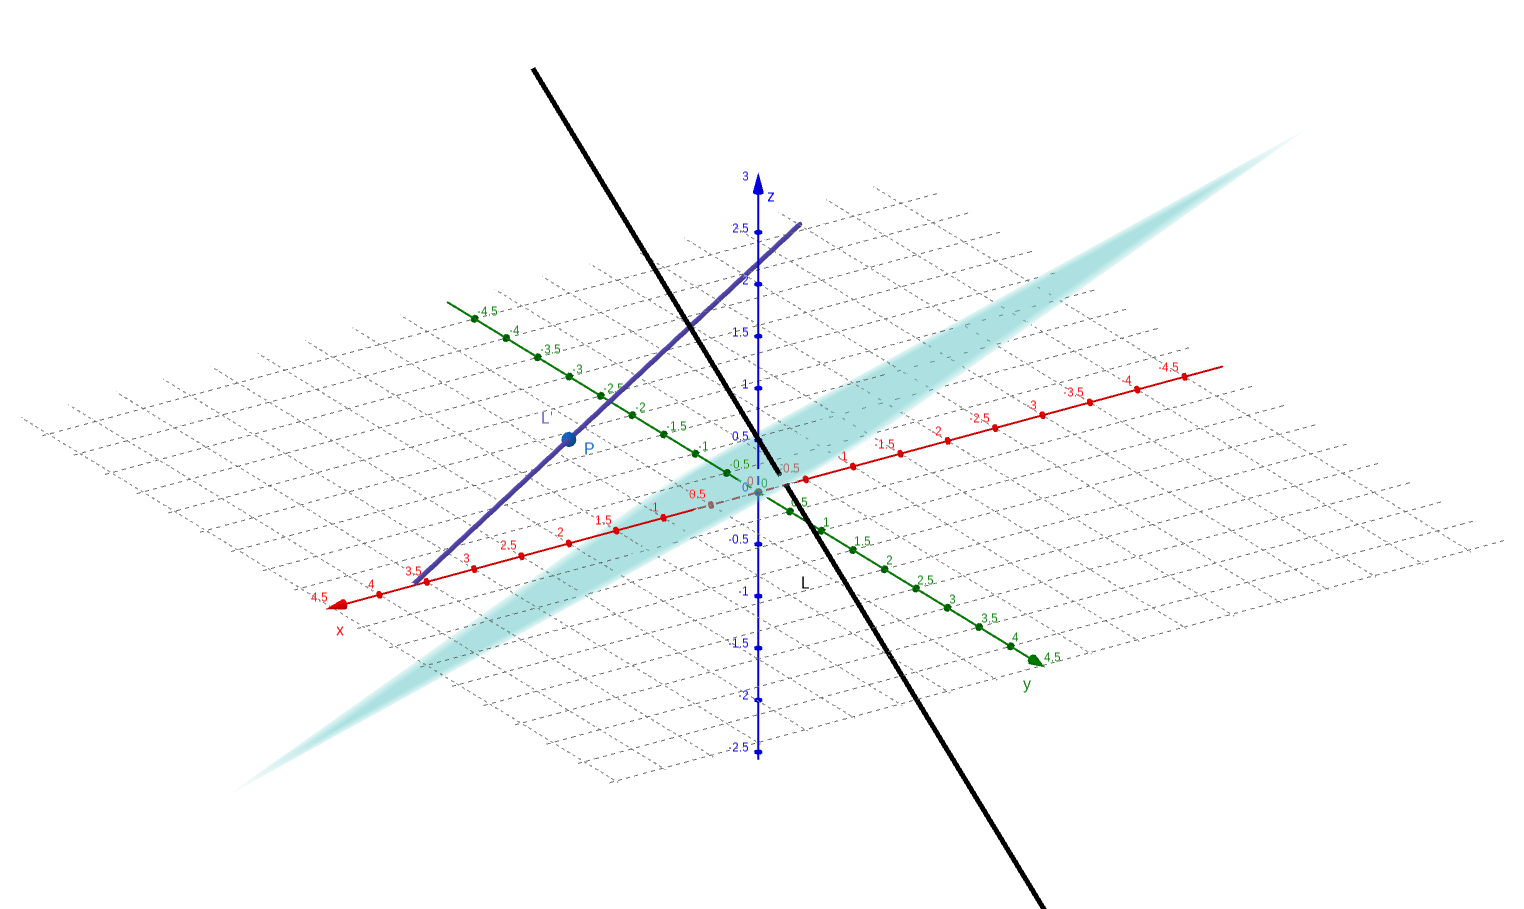
\includegraphics[width=15cm]{src/19_stuff.png}
            \caption{Grafica de \(\fancyL\), \(\fancyL'\), \(P\) y \(\fancyP\) del punto 19 en \(\realR^3\)}%
            \label{pt-nineteen-graph}
        \end{figure}
\setcounter{enumi}{20}
\item Sean \(\fancyL_1, \fancyL_2, \fancyP_1, \fancyP_2\) las rectas y planos cuyas ecuaciones son las siguientes:
    \[
        \begin{aligned}
            \fancyL_1 &: -x = \frac{y - 2}{4} = \frac{z + 1}{-2}
            \hspace{1cm}
            &\fancyL_2: 
            \begin{cases}
                x = -1 -2t \\
                y = 4 +8t \\ 
                z = -2 -4t \\
            \end{cases} 
            \\
            \fancyP_1 &:
            \begin{cases}
                x = -2t \\
                y = 2 - s \\
                z = t - 2s
            \end{cases}
            \hspace{1cm}
            &\fancyP_2: -x + 4y - 2z = 8
            \\
        \end{aligned}
    \]
    \begin{itemize}
        \item Si \(Q = \left(\begin{smallmatrix}1 \\ −2 \\ 1\end{smallmatrix}\right)\) se puede decir que:
            \begin{itemize}
                \item \(Q \in \fancyL_1\) \\
                    Si \(Q\) es un punto en \(\fancyL\), al estar la recta en sus ecuaciones simétricas, se debe mantener la igualdad al 
                    reemplazar \(x, y, z\) por cada componente de \(Q\).
                    \[
                        \begin{aligned}
                            -(1) &= \frac{(-2) -2}{4} &= \frac{(1) + 1}{-2} \\
                            -1 &= \frac{-4}{4} &= \frac{2}{-2} \\
                            -1 &= -1 &= -1 \\
                        \end{aligned}
                    \]
                    Como la igualdad se mantiene, podemos afirmar que \(Q\) es un punto en \(\fancyL_1\).
                \item \(Q \in \fancyL_2\) \\
                    De manera análoga, podemos reemplazar a \(x, y, z\) en \(\fancyL_2\) por cada componente de \(Q\), sin embargo, ahora debemos mirar si 
                    \(t\) es consistente en el sistema de ecuaciones, ya que \(\fancyL_2\) esta en sus ecuaciones parámetricas.
                    \[
                        \begin{cases}
                            1 = -1 -2t \\
                            -2 = 4 +8t \\ 
                            1 = -2 -4t
                        \end{cases}
                        \begin{cases}
                            2 = -2t \\
                            -6 = 8t \\ 
                            3 = -4t
                        \end{cases}
                        \begin{cases}
                            -1 = t \\
                            -\frac{3}{4} = t \\ 
                            -\frac{3}{4} = t
                        \end{cases}
                    \]
                    Como \(t\) no es consistente en el sistema de ecuaciones, se tiene que \(Q\) no es un punto en \(\fancyL_2\).
                \item \(Q \in \fancyP_1\) \\
                    Si \(Q\) esta en el plano \(\fancyP_1\), deben existir \(t\) y \(s\) tal que en las ecuaciones parámetricas del plano sean consistentes.
                    \[
                        \begin{cases}
                            1 = -2t \\
                            -2 = 2 - s \\
                            1 = t - 2s
                        \end{cases}
                        \begin{cases}
                            -\frac{1}{2} = t \\
                            4 = s \\
                            1 = -\frac{1}{2} - 8 = -\frac{17}{2}
                        \end{cases}
                    \]
                    Al verificar si \(Q\) esta en el plano, se pudo despejar a \(t\) y \(s\) en la 1\tsup{ra} y 2\tsup{da} ecuaciones, sin embargo, 
                    al reemplazar estas variables en la 3\tsup{ra} ecuación se obtiene una inconsistencia.
                    Por ende \(Q\) no es un punto en el plano \(\fancyP_1\).
                \item \(Q \in \fancyP_2\) \\
                    Si \(Q\) es un punto en el plano \(\fancyP_2\), al estar en su ecuación normal, se va a tener que si reemplazamos a \(x, y, z\) por 
                    cada componente de \(Q\), y se mantiene la igualdad, \(Q\) va a estar en \(\fancyP_2\). Verifiquemos esto
                    \[
                        \begin{aligned}
                            -(1) + 4(-2) -2(1) &= 8 \\
                            -1 -8 -2 &= 8 \\
                            -13 &= 8 \\
                        \end{aligned}
                    \]
                    Como no se mantiene la igualdad, se tiene que \(Q \not\in \fancyP_2\)
            \end{itemize}
        \item La recta \(\fancyL_2\) y el plano \(\fancyP_2\) se interceptan en:
            \begin{itemize}
				\item Ningún punto
				\item Un punto
				\item Infinitos puntos
				\item N.A
            \end{itemize}
        \item De las rectas \(\fancyL_1\) y \(\fancyL_2\) se puede decir que:
            \begin{itemize}
                \item \(\fancyL_1 \perp \fancyL_2\) \\
                    Si \(\fancyL_1\) es ortogonal a \(\fancyL_2\) entonces al hacer producto punto por ambos vectores directores el resultado debe ser cero.
                    \[
                        d_1 \cdot d_2 =
                        \begin{pmatrix}
                            -1 \\ 4 \\ -2
                        \end{pmatrix}
                        \cdot
                        \begin{pmatrix}
                            -2 \\ 8 \\ -4
                        \end{pmatrix}
                        =
                        (-1 \cdot -2) + (4 \cdot 8) + (-2 \cdot -4)
                        =
                        2 + 32 + 8
                        =
                        42
                        \neq
                        0
                    \]
                    Como \(d_1 \cdot d_2 \neq 0\), entonces ambas rectas no son ortogonales.
                \item \(\fancyL_1 \parallel \fancyL_2\) \\
                    Si \(\fancyL_1 \parallel \fancyL_2\) entonces, siendo \(d_1\) y \(d_2\) los vectores directores de las rectas, se va a tener que
                    \(d_1 \times d_2 = \vec{0}\). Verifiquemos esta afirmación.
                    \[
                        d_1 \times d_2
                        =
                        \begin{pmatrix}
                            -1 \\ 4 \\ -2
                        \end{pmatrix}
                        \times
                        \begin{pmatrix}
                            -2 \\ 8 \\ -4
                        \end{pmatrix}
                        =
                        \begin{pmatrix}
                            (4 \cdot -4) - (-2 \cdot 8) \\
                            -\left( (-1 \cdot -4) - (-2 \cdot -2) \right) \\
                            (-1 \cdot 8) - (4 \cdot -2)
                        \end{pmatrix}
                        =
                        \begin{pmatrix}
                            -16 + 16 \\
                            -4 + 4 \\
                            -8 + 8
                        \end{pmatrix}
                        =
                        \begin{pmatrix}
                            0 \\ 0 \\ 0
                        \end{pmatrix}
                        = 
                        \vec{0}
                    \]
                    Entonces, como \(d_1 \times d_2 = \vec{0}\), vamos a tener que \(\fancyL_1\) y \(\fancyL_2\) son paralelas.
                \item \(\fancyL_1 \cap \fancyL_2 \neq \emptyset\) \\
                    Ya sabemos que \(\fancyL_1\) es paralela con \(\fancyL_2\) por el caso anterior, entonces podemos mirar si o
                    \(\fancyL_1 \cap \fancyL_2 = \emptyset\) o \(\fancyL_1 = \fancyL_2\), lo cual se puede verificar viendo que, 
                    si ambas rectas contienen un mismo punto y no se tiene ninguna inconsistencia. Para esto, sea 
                    \[
                        P = \begin{pmatrix}
                            p_1 \\ p_2 \\ p_3
                        \end{pmatrix}
                        \hspace{0.5cm}
                        \fancyL_1:
                        \begin{cases}
                            x = -t \\
                            y = 2 + 4t \\
                            z = -1 -2t 
                        \end{cases}
                        t \in \realR
                        \hspace{0.5cm}
                        \fancyL_2:
                        \begin{cases}
                            x = -1 -2s \\
                            y = 4 + 8s \\
                            z = -2 -4s 
                        \end{cases}
                        s \in \realR
                    \]
                    \[
                        \left\{
                        \begin{aligned}
                            -t = &p_1 = -1 -2s \\
                            2 + 4t = &p_2 = 4 + 8s \\
                            -1 -2t = &p_3 = -2 -4s 
                        \end{aligned}
                        \right.
                        \hspace{0.5cm}
                        \left\{
                        \begin{aligned}
                            t &= 1 +2s \\
                            4t &= 2 + 8s \\
                            -2t &= -1 -4s 
                        \end{aligned}
                        \right.
                        \left\{
                        \begin{aligned}
                            t &= 1 +2s \\
                            t &= \frac{1}{2} + 2s \\
                            t &= \frac{1}{2} + 2s 
                        \end{aligned}
                        \right.
                        \hspace{0.5cm}
                    \]
                    Como \(t\) es inconsistente, \(t = 1 + 2s\) y \(t = \frac{1}{2} + 2s\), vamos a tener que las rectas \(\fancyL_1\) y \(fancyL_2\) no se cortan en ningún punto,
                    es decir \(\fancyL_1 \cap \fancyL_2 = \emptyset\) y al ser paralelas también se puede afirmar con esto que \(\fancyL_1 \neq \fancyL_2\).
                \item \(\fancyL_1 \nparallel \fancyL_2\) \\
                    Por el proceso hecho en el caso anterior, se puede afirmar que \(\fancyL_1 \parallel \fancyL_2\).
            \end{itemize}
        \item De los planos \(\fancyP_1\) y \(\fancyP_2\) se puede decir que:
            \begin{itemize}
                \item \(\fancyP_1 \perp \fancyP_2\) \\
                    Si los planos \(\fancyP_1\) y \(\fancyP_2\) son ortogonales, vamos a tener que apartir de sus vectores normales \(n_1\) y \(n_2\) 
                    van a ser ortogonales. Aunque debemos saber el vector normal de cada plano. Para esto, \(\fancyP_2\) al estar en su ecuación normal,
                    va a ser bastante sencillo obtener su vector normal, sin embargo para \(\fancyP_1\), debemos hacer producto cruz entre ambos vectores directores
                    para así obtener su vector normal.
                    \[
                        n_1 = 
                        \begin{pmatrix}
                            -2 \\ 0 \\ 1
                        \end{pmatrix}
                        \times
                        \begin{pmatrix}
                            0 \\ -1 \\ -2
                        \end{pmatrix}
                        =
                        \begin{pmatrix}
                            (0 \cdot -2) - (1 \cdot -1) \\
                            -( (-2 \cdot -2) - (1 \cdot 0) ) \\
                            (-2 \cdot -1) - (0 \cdot 0)
                        \end{pmatrix}
                        =
                        \begin{pmatrix}
                            0 + 1 \\
                            -4 + 0 \\
                            2 + 0
                        \end{pmatrix}
                        =
                        \begin{pmatrix}
                            1 \\ -4 \\ 2
                        \end{pmatrix}
                    \]
                    Ahora con ambos vectores normales, verificamos si son ortogonales.
                    \[
                        n_1 \cdot n_2 
                        =
                        \begin{pmatrix}
                            1 \\ -4 \\ 2
                        \end{pmatrix}
                        \cdot
                        \begin{pmatrix}
                            -1 \\ 4 \\ -2
                        \end{pmatrix}
                        =
                        (1 \cdot -1) + (-4 \cdot 4) + (2 \cdot -2)
                        =
                        -1 - 16 - 4
                        =
                        -21
                        \neq
                        0
                    \]
                    Como \(n_1 \cdot n_2 \neq 0\), vamos a tener que \(\fancyP_1\) y \(\fancyP_2\) no son ortogonales.
                \item \(\fancyP_1 \nparallel \fancyP_2\) \\
                    Si ambos planos no son paralelos, entonces el producto cruz de sus vectores normales no va a ser igual al vector nulo o vector cero. Verifiquemos esta afirmación
                    \[
                        n_1 \times n_2 
                        =
                        \begin{pmatrix}
                            1 \\ -4 \\ 2
                        \end{pmatrix}
                        \times
                        \begin{pmatrix}
                            -1 \\ 4 \\ -2
                        \end{pmatrix}
                        =
                        \begin{pmatrix}
                            (-4 \cdot -2) - (2 \cdot 4) \\
                            -( (1 \cdot -2) - (2 \cdot -1) ) \\
                            (1 \cdot 4) - (-4 \cdot -1)
                        \end{pmatrix}
                        =
                        \begin{pmatrix}
                            8 - 8 \\
                            2 - 2 \\ 
                            4 - 4
                        \end{pmatrix}
                        =
                        \begin{pmatrix}
                            0 \\ 0 \\ 0
                        \end{pmatrix}
                        =
                        \vec{0}
                    \]
                    Dado a que el producto cruz de ambos vectores normales es igual al vector cero, vamos a tener que ambos planos son paralelos, es decir 
                    que la afirmación dada es falsa.
                \item \(\fancyP_1 \cap \fancyP_2 = \emptyset\) \\
                    Taniendo en cuenta que los planos \(\fancyP_1\) y \(\fancyP_2\) son paralelos, podemos verificar si la intersección entre ambos planos es infinita, 
                    es decir \(\fancyP_1 = \fancyP_2\), o si la intersección es vacía, es decir \(\fancyP_1 \cap \fancyP_2 = \emptyset\).
                    Podemos verificar que \(\fancyP_1 = \fancyP_2\) teniendo que \(\fancyP_1 \parallel \fancyP_2\), simplemente viendo si para un punto \(P\) se comparte
                    en ambos planos. Sin embargo, antes de verificar esto vamos a necesitar que \(\fancyP_2\) este en sus ecuaciones parámetricas, para simplificar el proceso.
                    Para esto, vamos a necesitar encontrar dos vectores directores, \(t_2\) y \(s_2\), de \(\fancyP_2\), tal que \(\left\{t_2, s_2\right\}\) sea \(l.i\) y 
                    \(t_2 \cdot n = 0 = n \cdot s_2\). Entonces
                    \[
                        t_2 = 
                        \begin{pmatrix}
                            -2 \\ 1 \\ 1
                        \end{pmatrix}
                        \hspace{0.5cm}
                        s_2  =
                        \begin{pmatrix}
                            0 \\ 3 \\ 6
                        \end{pmatrix}
                    \]
                    Si \(V = \left\{t_2, s_2\right\}\) es \(l.i\) entonces los únicos escalares tal que una combinación lineal de \(V\) sea igual a \(\vec{0}\) van a ser \(\lambda_1 = \lambda_2 = 0\).
                    Esto se puede ver de la siguiente forma 
                    \[
                        \lambda_1 
                        \begin{pmatrix}
                            -2 \\ -1 \\ -1
                        \end{pmatrix}
                        +
                        \lambda_2
                        \begin{pmatrix}
                            0 \\ 3 \\ 6
                        \end{pmatrix}
                        =
                        \vec{0};
                        \hspace{0.5cm}
                        \begin{cases}
                            -2\lambda_1  = 0 \\
                            \lambda_1 + 3\lambda_2 = 0 \\
                            \lambda_1 + 6\lambda_2 = 0
                        \end{cases}
                    \]
                    Lo cual lo podemos tomar como una matriz explandida \(\left(A\mid\vec{0}\right)\) donde \(A\) es la matriz de coeficientes del sistema de ecuaciones lineales. 
                    Entonces apartir de operaciones elementales veamos si este sistema tiene una única solución.
                    \[
                        \begin{pmatrix}
                            -2 & 0 \\
                            1 & 3 \\
                            1 & 6 \\
                        \end{pmatrix}
                        \sim
                        \begin{aligned}
                            -\frac{1}{2}F_1 &\mapsto F_1 \\
                            F_3 - F_2 &\mapsto F_3 \\
                            \frac{1}{3}F_3 &\mapsto F_3 
                        \end{aligned}
                        \begin{pmatrix}
                            1 & 0 \\
                            1 & 3 \\
                            0 & 1 \\
                        \end{pmatrix}
                        \sim
                        \begin{aligned}
                            F_2 &\leftrightarrow F_3 \\
                            F_3 - F_1 &\mapsto F_3 \\
                            F_3 - 3F_2 &\mapsto F_3 \\
                        \end{aligned}
                        \begin{pmatrix}
                            1 & 0 \\
                            0 & 1 \\
                            0 & 0 \\
                        \end{pmatrix}
                    \]
                    Entonces por la 1\tsup{ra} fila sabemos que \(\lambda_1\) es igual a cero, y por la 2\tsup{da} fila, de manera similar, \(\lambda_2\) también es igual a cero.
                    Entonces el conjunto de ambos vectores directores es \(l.i\). Ahora verifiquemos que sean ortogonales al vector normal del plano.
                    \[
                        t_1 \cdot n =
                        \begin{pmatrix}
                            -2 \\ -1 \\ -1
                        \end{pmatrix}
                        \cdot
                        \begin{pmatrix}
                            -1 \\ 4 \\ -2
                        \end{pmatrix}
                        =
                        (-2 \cdot -1) + (-1 \cdot 4) + (-1 \cdot -2)
                        =
                        2 - 4 + 2 
                        =
                        0
                    \]
                    \[
                        s_1 \cdot n =
                        \begin{pmatrix}
                            0 \\ 3 \\ 6
                        \end{pmatrix}
                        \cdot
                        \begin{pmatrix}
                            -1 \\ 4 \\ -2
                        \end{pmatrix}
                        =
                        (0 \cdot -1) + (3 \cdot 4) + (6 \cdot -2)
                        =
                        0 + 12 - 12
                        =
                        0
                    \]
                    Al tener todo lo necesario para poder definir el plano \(\fancyP_3\) en sus ecuaciones parámetricas, teniendo un punto en el plano \(\left(\begin{smallmatrix}0 \\ 2 \\ 0\end{smallmatrix}\right)\), 
                    podemos definirlo como
                    \[
                        \fancyP_2: \begin{cases}
                            x = -2t \\
                            y = 2 -t + 3s \\
                            z = -t + 6s
                        \end{cases}
                        \hspace{0.5cm}
                        \begin{pmatrix}
                            0 \\ 2 \\ 0
                        \end{pmatrix}
                        \in
                        \fancyP_2
                        \text{ ya que: }
                        \begin{aligned}
                            -(0) + 4(2 -2(0) &= 8 \\
                            8 &= 8 \\
                        \end{aligned}
                    \]
                    Ahora, volviendo a nuestro problema inicial, vamos a ver si para un \(P\) arbitrario tal que este en ambos planos, sin que estos presenten alguna inconsistencia.
                    \[
                        P = 
                        \begin{pmatrix}
                            p_1 \\ p_2 \\ p_3
                        \end{pmatrix};
                        \hspace{0.5cm}
                        \fancyP_1:
                        \begin{cases}
                            x = -2t \\
                            y = 2 - s \\
                            z = t - 2s
                        \end{cases};
                        \hspace{0.5cm}
                        \fancyP_2:
                        \begin{cases}
                            x = -2t \\
                            y = 2 -t + 3s \\
                            z = -t + 6s
                        \end{cases}
                    \]
                    \[
                        \begin{cases}
                            -2t = p_1 = -2t \\
                            2 - s = p_2 = 2 -t + 3s \\
                            t - 2s = p_3 = -t + 6s
                        \end{cases}
                        \hspace{0.5cm}
                        \begin{cases}
                            -2t = -2 -2t \\
                            2 - s = 2 -t + 3s \\
                            t - 2s = -t + 6s
                        \end{cases}
                        \hspace{0.5cm}
                        \begin{cases}
                            -2t = -2t \\
                            2 - s = 2 -t + 3s \\
                            t - 2s = -t + 6s
                        \end{cases}
                        \hspace{0.5cm}
                        \begin{cases}
                            t = t \\
                            \frac{t}{4} = s \\
                            \frac{2t}{8} = \frac{t}{4} = s
                        \end{cases}
                    \]
                    Como tenemos que el sistema de ecuaciones parámetricas es consistente, el punto \(P\) esta en ambos planos, y al ser estos paralelos y compartir almenos un punto,
                    vamos a tener que ambos planos son iguales. Es decir \(\fancyP_1 = \fancyP_2\)
                \item \(\fancyP_1 = \fancyP_2\) \\
                    En el punto anterior se demostro que ambos planos son iguales al compartir almenos un punto y ser paralelos. Sin embargo, puede ver la grafica de los planos, rectas y puntos de este ejercicio en 
                    la Figura-\ref{pt-twentyone-graph}           
                    \begin{figure}
                        \centering
                        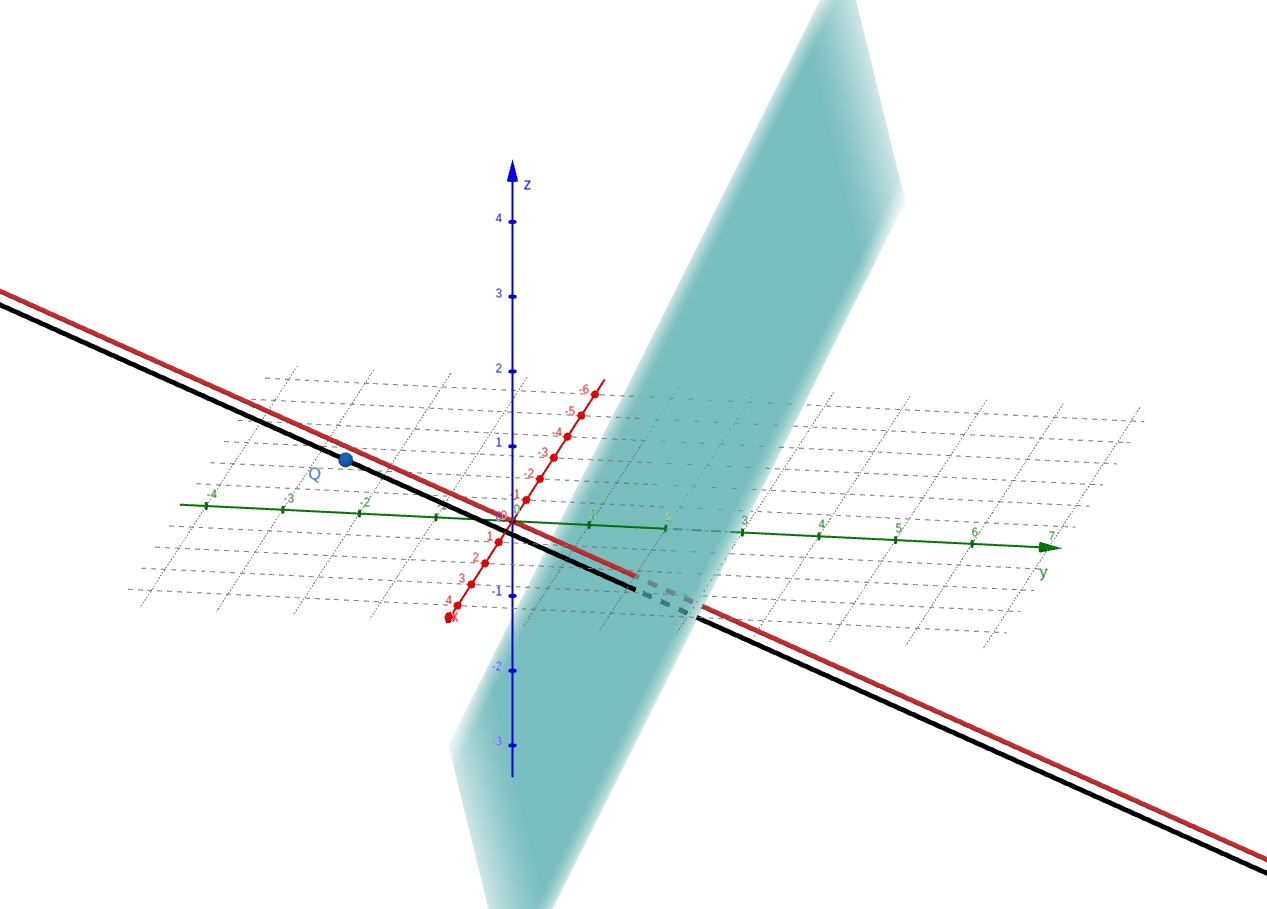
\includegraphics[width=15cm]{src/21_graph.png}
                        \caption{Grafica de \(\fancyL_1, \fancyL_2, \fancyP_1, \fancyP_2\) y \(Q\) del punto 21 en \(\realR^3\)}%
                        \label{pt-twentyone-graph}
                    \end{figure}
            \end{itemize}
    \end{itemize}
\end{enumerate}
\end{document}
